\chapter{Resultaten}

In dit hoofdstuk worden de bevindingen van de uitgevoerde Proof of Concept (PoC) gepresenteerd en getoetst aan de evaluatiecriteria die in hoofdstuk~\ref{ch:Evaluatie} zijn vastgelegd. De resultaten zijn enerzijds gebaseerd op de geautomatiseerde aanvalssimulaties en handmatige testen, en anderzijds op de gegenereerde telemetrie in de dashboards van de Akamai Firewall for AI en Dynatrace.

\section{Correctheid (Detectienauwkeurigheid)}

De primaire doelstelling van de Firewall is het effectief neutraliseren van applicatielaag-dreigingen en LLM-specifieke kwetsbaarheden, zonder legitiem verkeer onnodig te verstoren.\\

Tijdens de testfase zijn de geautomatiseerde Bash-scripts (zoals beschreven in sectie~5.5) succesvol afgevuurd op de on-premise infrastructuur. Uit de algemene resultaten blijkt dat de Akamai's Firewall for AI in staat is om de JSON-payloads accuraat te ontleden en kwaadaardige invoer proactief te blokkeren (True Positives).

\subsection{Samenvatting van de geteste use-cases (True Positives)}

Om de correctheid van de Firewall structureel te valideren, zijn alle acht use-cases uit de risicoanalyse onderworpen aan gesimuleerde aanvallen. Aangezien de firewall is geconfigureerd om bij elke regelovertreding in de preventieve modus in te grijpen, resulteerde elke succesvolle detectie in een blokkade.

\begin{table}[h]
    \centering
    \caption{Overzicht van de uitgevoerde aanvalssimulaties en de resulterende Firewall-for-AI-blokkades}
    \label{tab:waf-results}
    \begin{tabular}{|l|l|l|l|}
        \hline
        \textbf{Categorie} & \textbf{Use-Case} & \textbf{Payload / Testmethode} & \textbf{Resultaat} \\ \hline
        Input & Code detected & SQLi (' OR 1=1) en XSS (<script>) & Succes (HTTP 403) \\ \hline
        Input & Input too long & String >256 karakters & Succes (HTTP 403) \\ \hline
        Input & Non-allowed language & Russische prompt & Succes (HTTP 403) \\ \hline
        Input & Toxic content & Agressieve taal & Succes (HTTP 403) \\ \hline
        Input & PII detected & IBAN & Succes (HTTP 403) \\ \hline
        Output & PII detected & besmet database-record & Succes (HTTP 403) \\ \hline 
        Output & Output too long & specifieke test prompt & Succes (HTTP 403) \\ \hline 
        Output & Code detected & Besmet database-record & Succes (HTTP 403) \\ \hline 
        Output& Toxic content & Agressieve taal (stored in DB) & Succes (HTTP 403) \\ \hline 
    \end{tabular}
\end{table}

\subsection{Visueel bewijs van interventie}

Om de mechanismen achter de in Tabel~\ref{tab:waf-results} genoteerde successen te verifiëren, is het cruciaal om de incidenten vanuit twee perspectieven te belichten: het standpunt van de aanvaller en dat van de verdedigende infrastructuur.\\

Wanneer het Bash-script een malafide payload verstuurt (bijvoorbeeld Toxic content), verbreekt de Firewall de verbinding voordat deze de Nginx-gateway bereikt. Listing~\ref{lst:waf403} toont de respons die de aanvaller ontvangt.

\begin{lstlisting}[language={}, caption={Terminal-output na een WAF-blokkade}, label={lst:waf403}, breaklines=true, numbers=left,frame=singl]
{
    "ai_firewall": "block",
    "reason": "Code_injection",
    "message": "Code detected in input!"
}
\end{lstlisting}

Wanneer we vervolgens in de Web Security Analytics van Akamai gaan kijken zien we het volgende:

\begin{figure}[H]
    \centering
    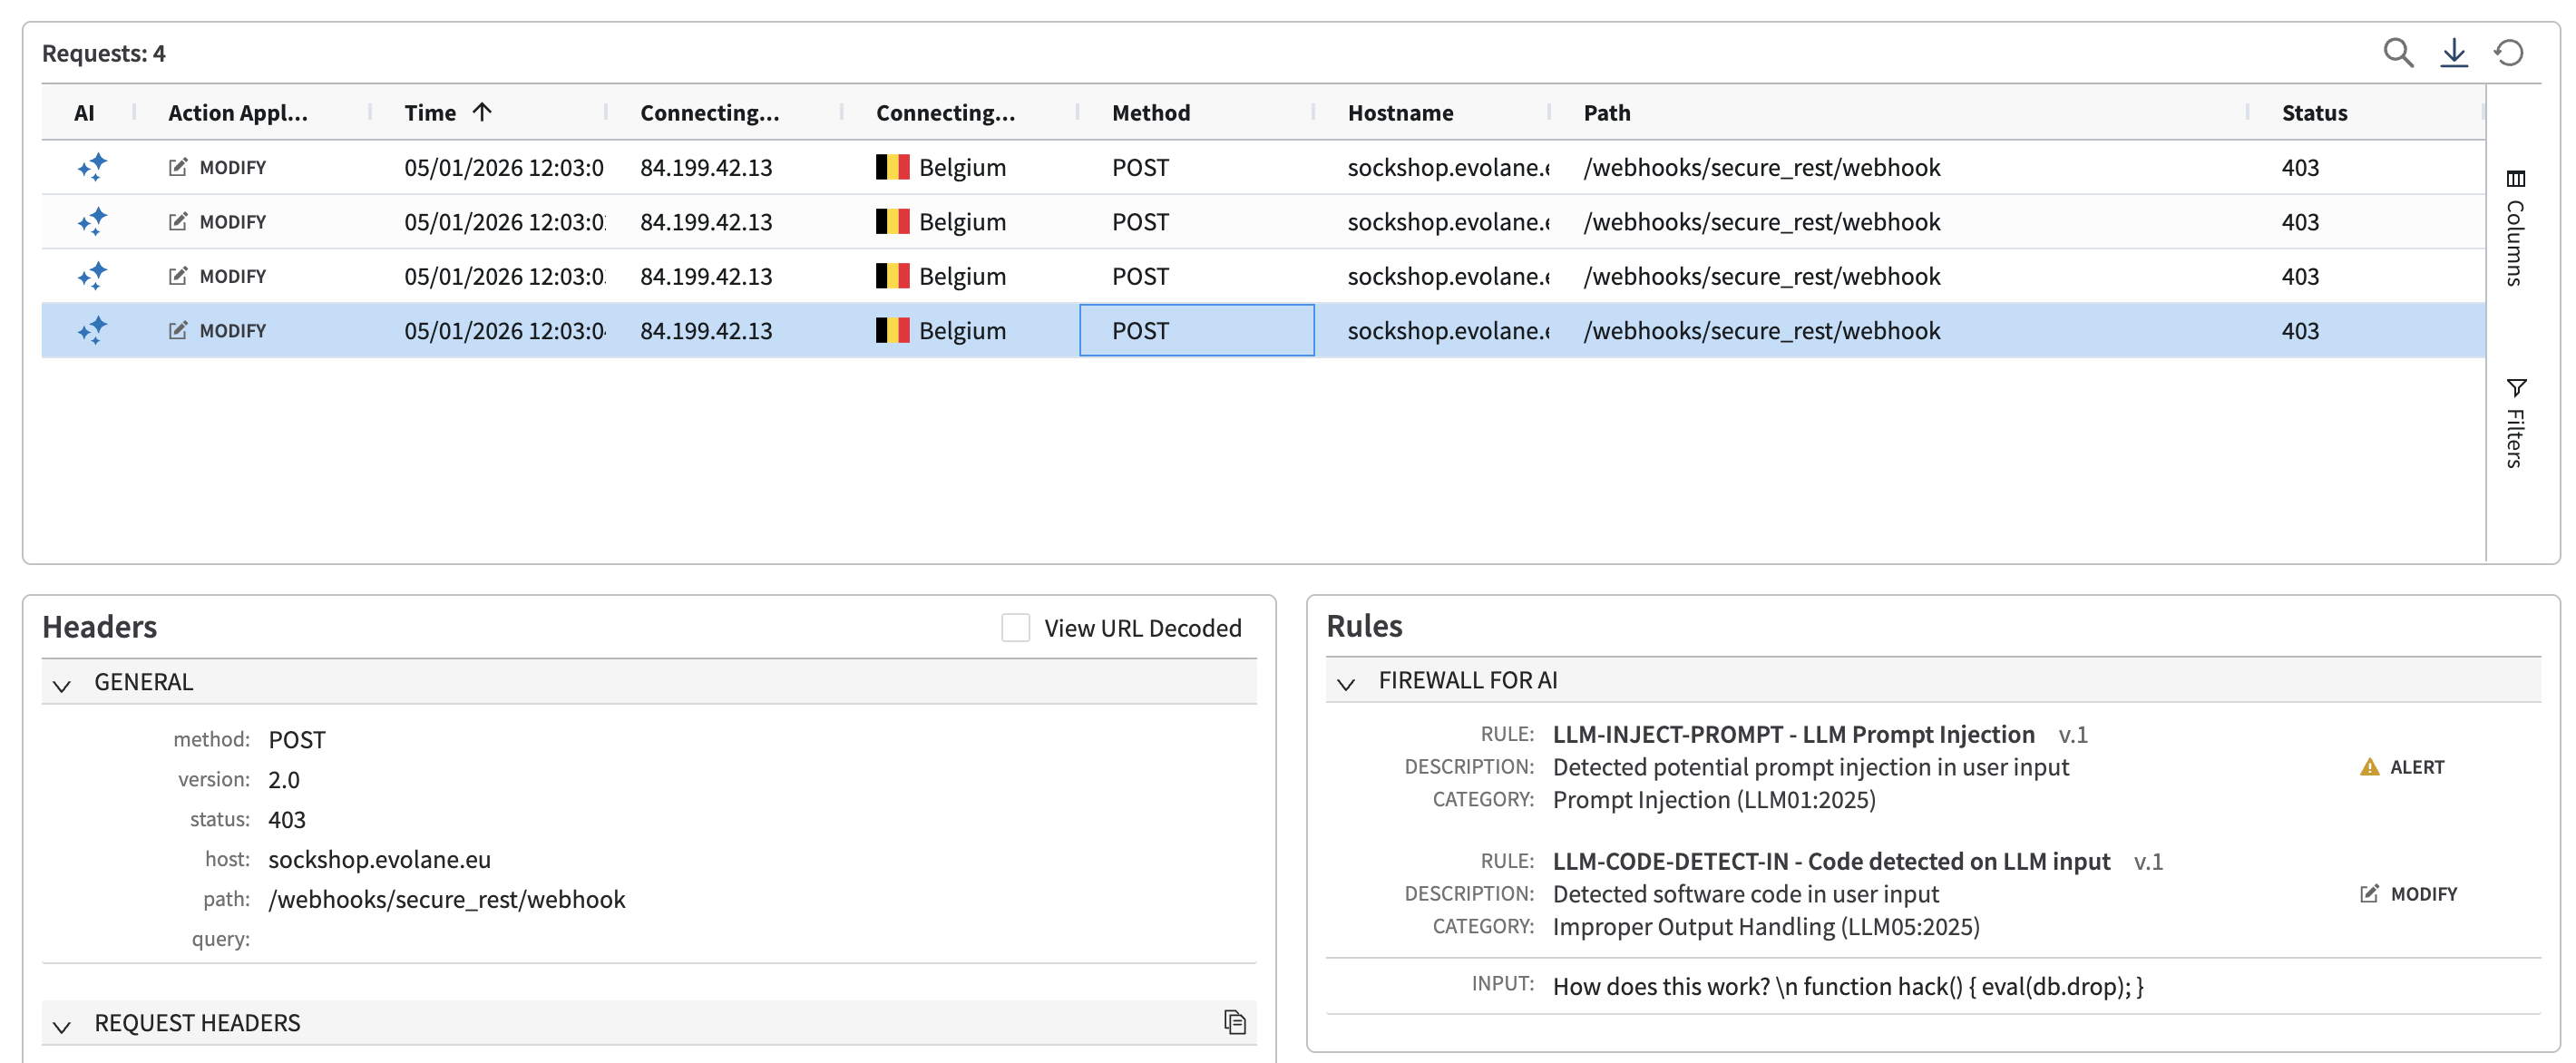
\includegraphics[width=1\linewidth]{img/wsa403.png}
    \caption{Incidentenregistratie in het Akamai-dashboard}
    \label{fig:akamai-dashboard}
\end{figure}

\subsection{Beheer van False Positives en finetuning}

Hoewel de firewall effectief bleek, is het voorkomen van False Positives cruciaal.

\begin{itemize}
    \item [TODO:] False positives
    \item [TODO:]
\end{itemize}

Deze finetuning bewijst dat ook voor firewalls for AI calibratie nodig is om succesvol te zijn.

\section{Traceerbaarheid en Compliance}

TODO

\section{Gebruiksvriendelijkheid (SecOps perspectief)}

De beheerbaarheid is geëvalueerd vanuit het perspectief van de beheerder.

\subsection{Configuratiegemak (Akamai)}

Het configureren van JSONPath-inspecties binnen Akamai bleek intuïtief. Door eerst Monitor-modus te gebruiken, konden regels veilig worden getest. Alleen kon pad nog niet met een wildcard werken. Na meerdere pogingen heb ik dus uiteindelijk gekozen om een eigen custom REST channel te maken.

\subsection{Incidentenanalyse}

TODO

\subsection{Integratie en zichtbaarheid (Dynatrace)}

TODO